\documentclass[12pt]{report}
\usepackage[utf8]{inputenc} 
\usepackage[T1]{fontenc}
\usepackage[francais]{babel}
\usepackage{layout}
\usepackage{graphicx}

%page de garde 
\title{Report of the first Phase of the project}
\author{Pierre-Yves \bsc{Hervo} \\Polytech Nantes High school of Engineering }
\date{11\up{th} of July 2013}

\begin{document}
\maketitle

\begin{abstract}

The ICCMR laboratory launch a project to design a software which can synthesis human voice by giving it specific values. This global project will be divided into smaller project and perfect each time. I worked on the first step of the project: the launch of the project by developing a solution to recreate vowels. 

This report presents the work I have realised on my project from the beginning of my internship the 03\up{rd} of June to the end of the first Phase the 12\up{th}of July.

\end{abstract}
  
\tableofcontents

J'insère le premier \cite{ref}, le second \cite{ref2}, le troisième \cite{ref3}, le quatrième \cite{ref4}, le cinquième \cite{ref5} et le sixième \cite{ref6}.


\part{Overall}
\chapter{Presentation of the project}
\section{Quick introduction}
As I said in the introduction of this report, i worked on the first phase of the global project by designing and developing a software that is capable of recreating the human vowels.
But what is the purpose of this project and why do I only worked on vowels ?
Isn't there existing software to synthesise human sound ?

Before giving the answer I had to make a little recap on the voice synthesis
 
\section{Presentation of Voice Synthesis}
We will here study the human voice from a physical point of view.

The human voice are created by the combination of different organs in our body.
It started in the lungs by producing an airstream and then pass through different elements of the body to exit by the mouth. Among those elements we can quote for example the larynx, the vocal cords, the tongue, and so on...

Some of them are are represented in the Figure \ref{ImageHumanVoice} in the page \pageref{ImageHumanVoice}.


According to the position of this muscles, the sound produced will be different. For example if the vocal are tense or not, it will have an influence of the vibration of the voice and so on the sound. It is the same for all the organs previously described, the form they had during the passage of the airstream will have an impact on the final sound.

\begin{figure}
\begin{center}
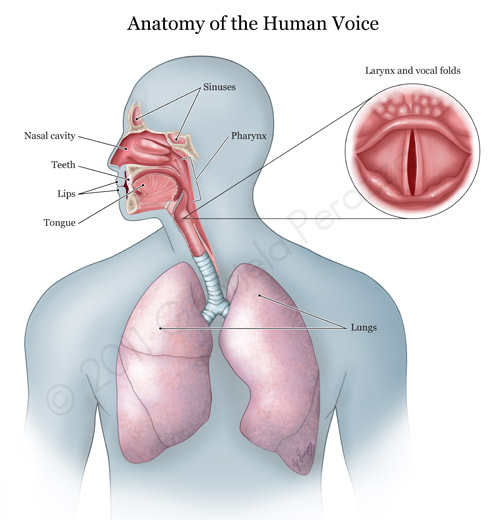
\includegraphics[scale=0.5]{human_voice.jpg} 
\end{center}
\caption{Some of the organs use in the voice synthesis process}
\label{ImageHumanVoice}
\end{figure}

There is some softwares that allows to create sound =. praat the best.

\section{Quick introduction}

\chapter{Presentation of Genetic algorithms}

\chapter{Presentation of Praat}

\part{Technical details}
\chapter{Praat Scripts}
\chapter{Presentation of watchmaker}
\chapter{Presentation of the basic manipulated Structures}
\chapter{result}
\appendix
\chapter{A scheme}

\listoffigures
\listoftables

\bibliographystyle{unsrt} 
\bibliography{bib} % mon fichier de base de données s'appelle bibli.bib
\end{document}